\documentclass[tikz,border=16pt]{standalone}
\usepackage{amsmath,amssymb}
\usepackage{tikz}
\usetikzlibrary{arrows.meta, positioning, calc, fit, backgrounds}

%% ---- palette (matches FSM figure) ----
\definecolor{cBlue}{RGB}{13,110,200}
\definecolor{cFillBlue}{RGB}{230,242,255}
\definecolor{cGray}{RGB}{95,108,120}
\definecolor{cFillGray}{RGB}{220,222,226}
\definecolor{cOrange}{RGB}{195,95,15}
\definecolor{cFillOrange}{RGB}{255,239,218}
\definecolor{cRed}{RGB}{170,35,35}
\definecolor{cFillRed}{RGB}{255,220,220}
\definecolor{cGreen}{RGB}{30,145,75}
\definecolor{cFillGreen}{RGB}{210,245,225}
\definecolor{cLegend}{RGB}{250,251,253}
\definecolor{cFillNeutral}{RGB}{245,246,248}

\tikzset{
  %% internal nodes
  inode/.style={rectangle, rounded corners=4pt, draw, minimum width=1.6cm,
                minimum height=0.55cm, font=\ttfamily\scriptsize, align=center,
                inner sep=3pt, line width=1.1pt},
  inodeB/.style={inode, draw=cBlue,   fill=cFillBlue,   text=cBlue},   % unchanged
  inodeO/.style={inode, draw=cOrange, fill=cFillOrange, text=cOrange}, % recomputed
  inodeG/.style={inode, draw=cGray,   fill=cFillGray,   text=cGray},   % root (before)
  inodeN/.style={inode, draw=cGreen,  fill=cFillGreen,  text=cGreen},  % root (after, new)
  %% leaf nodes
  leaf/.style={rectangle, rounded corners=3pt, draw, minimum width=1.3cm,
               minimum height=0.55cm, font=\ttfamily\scriptsize, align=center,
               inner sep=2pt, line width=1.1pt},
  leafB/.style={leaf, draw=cBlue,   fill=cFillBlue,  text=cBlue},
  leafR/.style={leaf, draw=cRed,    fill=cFillRed,   text=cRed},   % revoked
  leafX/.style={leaf, draw=cGray,   fill=cFillGray,  text=cGray,   dashed}, % removed
  leafO/.style={leaf, draw=cOrange, fill=cFillOrange,text=cOrange},% sibling in path
  %% edges
  edge/.style={draw=cGray!60, line width=1pt},
  pathedge/.style={draw=cOrange, line width=1.6pt},
}

\begin{document}
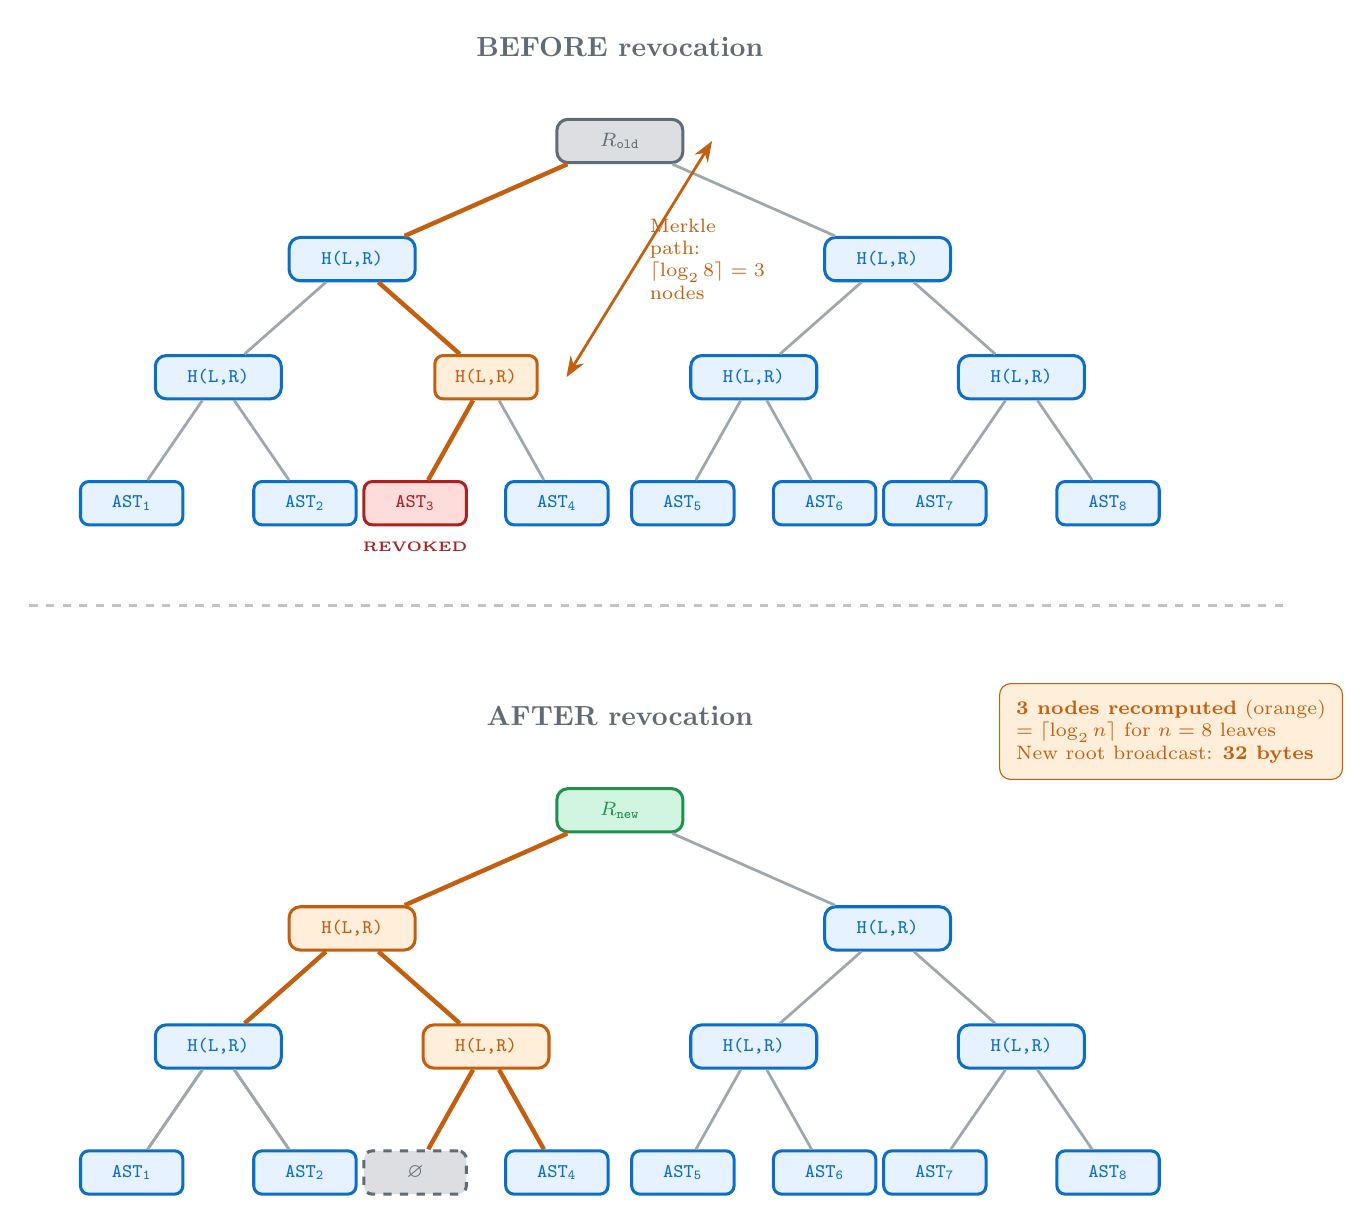
\begin{tikzpicture}

%% =============================================================
%%  BEFORE TREE  (top panel, origin at 0,0)
%% =============================================================

%% -- "BEFORE" label --
\node[font=\bfseries\normalsize, text=cGray] at (0, 1.2) {BEFORE revocation};

%% --- Level 0: root ---
\node[inodeG] (BRt) at (0, 0) {$R_{\text{old}}$};

%% --- Level 1 ---
\node[inodeB] (BL1) at (-3.4, -1.5) {\texttt{H(L,R)}};
\node[inodeB] (BR1) at ( 3.4, -1.5) {\texttt{H(L,R)}};

%% --- Level 2 ---
\node[inodeB]  (BLL2) at (-5.1, -3.0) {\texttt{H(L,R)}};
\node[leafO]   (BLR2) at (-1.7, -3.0) {\texttt{H(L,R)}};  %% sibling of revoked subtree
\node[inodeB]  (BRL2) at ( 1.7, -3.0) {\texttt{H(L,R)}};
\node[inodeB]  (BRR2) at ( 5.1, -3.0) {\texttt{H(L,R)}};

%% --- Level 3: leaves ---
\node[leafB] (L1) at (-6.2, -4.6) {\texttt{AST\textsubscript{1}}};
\node[leafB] (L2) at (-4.0, -4.6) {\texttt{AST\textsubscript{2}}};
\node[leafR] (L3) at (-2.6, -4.6) {\texttt{AST\textsubscript{3}}};   %% REVOKED
\node[leafB] (L4) at (-0.8, -4.6) {\texttt{AST\textsubscript{4}}};
\node[leafB] (L5) at ( 0.8, -4.6) {\texttt{AST\textsubscript{5}}};
\node[leafB] (L6) at ( 2.6, -4.6) {\texttt{AST\textsubscript{6}}};
\node[leafB] (L7) at ( 4.0, -4.6) {\texttt{AST\textsubscript{7}}};
\node[leafB] (L8) at ( 6.2, -4.6) {\texttt{AST\textsubscript{8}}};

%% -- normal edges --
\draw[edge] (BRt) -- (BL1);
\draw[edge] (BRt) -- (BR1);
\draw[edge] (BL1) -- (BLL2);
\draw[edge] (BL1) -- (BLR2);
\draw[edge] (BR1) -- (BRL2);
\draw[edge] (BR1) -- (BRR2);
\draw[edge] (BLL2) -- (L1);
\draw[edge] (BLL2) -- (L2);
\draw[edge] (BLR2) -- (L3);
\draw[edge] (BLR2) -- (L4);
\draw[edge] (BRL2) -- (L5);
\draw[edge] (BRL2) -- (L6);
\draw[edge] (BRR2) -- (L7);
\draw[edge] (BRR2) -- (L8);

%% -- Merkle PATH highlight (L3 -> BLR2 -> BL1 -> Rt) in ORANGE --
\draw[pathedge] (BRt) -- (BL1);
\draw[pathedge] (BL1) -- (BLR2);
\draw[pathedge] (BLR2) -- (L3);

%% -- revoked leaf label --
\node[cRed, font=\bfseries\tiny, below=2pt of L3] {REVOKED};

%% -- path annotation brace --
\draw[cOrange, <->, >=Stealth, line width=1pt]
  ([xshift=10pt]BRt.east) -- ([xshift=10pt]BLR2.east)
  node[midway, right, font=\scriptsize, text=cOrange, align=left]
    {Merkle\\path:\\$\lceil\log_2 8\rceil=3$\\nodes};

%% =============================================================
%%  DIVIDER (horizontal)
%% =============================================================
\draw[cGray!40, dashed, line width=1.2pt] (-7.5, -5.9) -- (8.5, -5.9);

%% =============================================================
%%  AFTER TREE  (bottom panel, shifted -8.5 in y)
%% =============================================================
\def\dy{-8.5}

%% -- "AFTER" label --
\node[font=\bfseries\normalsize, text=cGray] at (0, \dy+1.2) {AFTER revocation};

%% --- Level 0: root (NEW, green) ---
\node[inodeN] (ARt) at (0, \dy+0) {$R_{\text{new}}$};

%% --- Level 1 (left subtree recomputed, right unchanged) ---
\node[inodeO] (AL1) at (-3.4, \dy-1.5) {\texttt{H(L,R)}};   %% recomputed
\node[inodeB] (AR1) at ( 3.4, \dy-1.5) {\texttt{H(L,R)}};   %% unchanged

%% --- Level 2 ---
\node[inodeB]  (ALL2) at (-5.1, \dy-3.0) {\texttt{H(L,R)}};   %% unchanged
\node[inodeO]  (ALR2) at (-1.7, \dy-3.0) {\texttt{H(L,R)}};   %% recomputed (sibling of null)
\node[inodeB]  (ARL2) at ( 1.7, \dy-3.0) {\texttt{H(L,R)}};
\node[inodeB]  (ARR2) at ( 5.1, \dy-3.0) {\texttt{H(L,R)}};

%% --- Level 3: leaves ---
\node[leafB] (A1) at (-6.2, \dy-4.6) {\texttt{AST\textsubscript{1}}};
\node[leafB] (A2) at (-4.0, \dy-4.6) {\texttt{AST\textsubscript{2}}};
\node[leafX] (A3) at (-2.6, \dy-4.6) {$\varnothing$};              %% removed
\node[leafB] (A4) at (-0.8, \dy-4.6) {\texttt{AST\textsubscript{4}}};
\node[leafB] (A5) at ( 0.8, \dy-4.6) {\texttt{AST\textsubscript{5}}};
\node[leafB] (A6) at ( 2.6, \dy-4.6) {\texttt{AST\textsubscript{6}}};
\node[leafB] (A7) at ( 4.0, \dy-4.6) {\texttt{AST\textsubscript{7}}};
\node[leafB] (A8) at ( 6.2, \dy-4.6) {\texttt{AST\textsubscript{8}}};

%% -- normal edges (unchanged subtree) --
\draw[edge] (AR1) -- (ARL2);
\draw[edge] (AR1) -- (ARR2);
\draw[edge] (ALL2) -- (A1);
\draw[edge] (ALL2) -- (A2);
\draw[edge] (ARL2) -- (A5);
\draw[edge] (ARL2) -- (A6);
\draw[edge] (ARR2) -- (A7);
\draw[edge] (ARR2) -- (A8);

%% -- recomputed path edges --
\draw[pathedge] (ARt) -- (AL1);
\draw[pathedge] (AL1) -- (ALL2);
\draw[pathedge] (AL1) -- (ALR2);
\draw[pathedge] (ALR2) -- (A3);
\draw[pathedge] (ALR2) -- (A4);
\draw[edge] (ALL2) -- (A1);
\draw[edge] (ALL2) -- (A2);

%% also draw root -> right in normal style
\draw[edge] (ARt) -- (AR1);

%% -- recomputed annotation --
\node[draw=cOrange, fill=cFillOrange, rounded corners=4pt,
      font=\scriptsize, align=left, inner sep=6pt,
      text=cOrange]
  at (7.0, \dy+1) {%
    \textbf{3 nodes recomputed} (orange)\\
    $= \lceil\log_2 n\rceil$ for $n=8$ leaves\\
    New root broadcast: \textbf{32 bytes}};

%% =============================================================
%%  CRL comparison callout (bottom center)
%% =============================================================
% \node[draw=cGray!60, fill=cLegend, rounded corners=6pt,
%       inner sep=10pt, font=\scriptsize, align=left,
%       minimum width=5.5cm]
%   at (0, \dy-6.4) {%
%     \textbf{Revocation overhead comparison}\\[4pt]
%     \textbf{CRL (SCMS/X.509):}~~$O(n)$ broadcast\\
%     \quad grow with every revocation\\[3pt]
%     \textbf{Merkle update (ours):}~~$O(\log n)$ recompute\\
%     \quad broadcast only new root ($32$ bytes)};

\end{tikzpicture}
\end{document}